\documentclass[a4paper,oneside,12pt]{article}

\usepackage{custom}
\newcommand{\barg}{\si{\bar}\text{g}} 
\usepackage{setspace}
\usepackage{chemist}
\usepackage{fancyhdr} 
\usepackage{amsmath}
\fancyhf{}   
\fancyfoot[C]{\thepage}                     
\renewcommand\headrulewidth{0pt}
\pagestyle{fancy}

\begin{document}

\begin{titlepage}

\begin{center}
\Huge
\textbf{MAPR1400 - Projet en cinétique appliquée\\}
\vspace{0.5cm}
\huge
\textbf{Polymérisation du méthacrylate de méthyle\\}
\Large
\vspace{0.5cm}
\textbf{Année académique 2015-2016\\}
\begin{figure}[b!]
	\center
	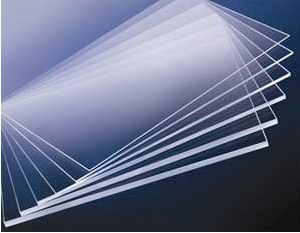
\includegraphics[width=12cm]{Images/plexi.jpg}
\end{figure}

\end{center}
\begin{figure}[b!]
\begin{Large}
\end{Large}
	DISPAS David, 7189-12-00\\
	PAQUET Arnaud, 3668-13-00\\
	\\
	\newline
	\center
	
\includegraphics[width=7cm]{Images/epl-logo.jpg}
\end{figure}
\end{titlepage}

\section{Applications du plexiglas dans la vie courante}

Le polyméthacrylate de méthyle (PMMA) est un polymère thermoplastique transparent. Plus connu sous le nom de plexiglas,...

\section{Evolution des concentrations}
La réaction que nous analysons est une polymérisation radicalaire. Elle peut donc être décomposée en les étapes suivantes:
\subsection{Amorçage}
L'amorceur utilisé est une molécule d'azobisisobutyronitrile (AIBN). 
\begin{equation}
	\ce{AIBN \underset{lent}{\xrightarrow{k_0}} N2 + 2A^\bullet}
\end{equation}	
La vitesse de décomposition de l'AIBN est très lente part rapport à celle de la seconde réaction. Seule une fraction f des radicaux créés est efficace pour réagir ensuite de la manière suivante:

\begin{equation}
\ce{A^{\bullet} + M \underset{rapide}{\xrightarrow{k_i}} R1} 
\end{equation}

où M est un monomère de MMA et $\ce{Rj}$ est une chaine en croissance composée d'un A auquel j monomères M se sont ajoutés. Nous pouvons utiliser l'hypothèse de quasi-stationnarité du radical (HQSR) $\frac{d[A^{\bullet}]}{dt}=0$ et ainsi obtenir que $2fk_{0}[AIBN]=k_{i}[A^{\bullet}][M]=r_i$.

\subsection{Propagation}
Les chaînes deviennent de plus en plus grandes en annexant des monomères. Pour une chaine de longueur 1 par exemple:
\begin{equation}
\ce{R1 + M \xrightarrow{k_p} R2}
\end{equation}
Nous pouvons généraliser pour une longueur arbitraire:
\begin{equation}
\ce{R_{j} + M \xrightarrow{k_p} R_{j+1}}
\end{equation}
Les $k_{p}$ de toutes les réactions de propagation sont considérés égaux, ce qui n'est théoriquement valable que pour des grandes chaines. Ceci est l'hypothèse d'équiréactivité de Flory.

\subsection{Terminaison}
Il existe deux types de terminaisons: la recombinaison et la dismutation. Travaillant à la température de 22.5°C, nous négligerons ici la seconde qui ne se produit qu'à plus haute température. La réaction de recombinaison est la suivante:

\begin{equation}
\ce{R_{n} + R_{m} \xrightarrow{k_t} P_{n+m}}
\end{equation}
où $P_{j}$ est une molécule de PMMA de longueur j. Pour simplifier, nous ferons l'hypothèse que $k_{t}$ ne dépend pas de la longueur des chaines.

\subsection{Transfert}
Nous disposons de plusieurs agents de transfert Tr pour lesquels nous connaissons les $C_{s}=\frac{k_{s}}{k_{p}}$. Ces derniers peuvent neutraliser une chaine et produire un radical qui pourra amorcer une nouvelle chaine:
\begin{equation}
\ce{R_{j} + TrH \xrightarrow{k_s} R_{j}H + Tr^{\bullet}}
\end{equation}

\begin{equation}
\ce{Tr^{\bullet} + M \xrightarrow{k_i,tr} R_{1}}
\end{equation}

Nous faisons l'hypothèse que $k_s$ est indépendant de la longueur des chaines.
\subsection{Calcul des lois de concentrations}
$\bullet$ Commençons par calculer la concentration en AIBN. Puisque le composé n'apparait que dans la première équation, l'expression de sa vitesse de disparition est simplement: $-\frac{d[AIBN]}{dt}=k_{0}[AIBN]$. On trouve aisément la solution: $$[AIBN]=[AIBN]_{t=0}e^{-k_{0}t} $$.\\

$\bullet$ La vitesse d'apparition globale des chaines R n'est autre que la somme des vitesses $r_{m}$ de chaque chaine $R_{m}$. Nous pouvons trouver que:
\begin{align*}
r_{1}=\frac{d[R_{1}]}{dt}=r_{i}+k_{i,tr}[Tr^{\bullet}][M]-k_p[R_{1}][M]-k_{t}[R_1]\sum\limits_{j=1}^\infty[R_j]-k_{s}[R_{1}][TrH]
\end{align*}

\begin{align*}
r_{2}=\frac{d[R_{2}]}{dt}=k_p[R_{1}][M]-k_p[R_{2}][M]-k_{t}[R_2]\sum\limits_{j=1}^\infty[R_j]-k_{s}[R_{2}][TrH]
\end{align*}

\begin{align*}
r_{m}=\frac{d[R_{m}]}{dt}=k_p[R_{m-1}][M]-k_p[R_{m}][M]-k_{t}[R_m]\sum\limits_{j=1}^\infty[R_j]-k_{s}[R_{m}][TrH]
\end{align*}

Par conséquent:

\begin{equation}
\sum\limits_{m=1}^\infty r_{m}=r_i+ k_{i,tr}[Tr^{\bullet}][M] -k_{t}\sum\limits_{m=1}^\infty [R_m] \sum\limits_{j=1}^\infty[R_j]-k_{s}\sum\limits_{m=1}^\infty[R_{m}][TrH]
\end{equation}
L'HQSR appliquée sur $Tr^{\bullet}$ nous donne: $\frac{d[Tr^{\bullet}]}{dt}=0=k_{i,tr}[Tr^{\bullet}][M]-k_{s}\sum\limits_{m=1}^\infty[R_{m}][TrH]$. Nous pouvons donc simplifier notre expression. De plus, $\sum\limits_{j=1}^\infty[R_j] = [R]$:

\begin{equation}
\sum\limits_{m=1}^\infty r_{m}=r_i-k_{t}[R]^2
\end{equation}

Finalement, l'HQSR utilisée sur les radicaux R nous permet de dire que $\sum\limits_{m=1}^\infty r_{m}=0$ et donc que $r_i=k_{t}[R]^2=2fk_{0}[AIBN]$. La concentration en R est alors:

$$[R]=(\frac{2fk_{0}[AIBN]}{k_t})^{\frac{1}{2}}$$\\

$\bullet$Passons maintenant à la concentration en monomères M. La vitesse de disparition de M est $r_M = -\frac{d[M]}{dt}=r_{i}+k_{i,tr}[M][Tr^{\bullet}]+k_{p}[M][R]$


\section{Influence des différents effets observés}

\section{Epuisement de l'amorceur}

\section{Effets de la température}

\end{document}
